\section{Mozart/Oz}
\verb= $Id$ =

Mozart is an implementation of the multiparadigmatic language Oz. Oz is functional
language with built-in support for threaded applications and paralelisation. It also
contains support for constraint solving. It also supported to run subroutines on computers
connected to the cluster. Since it is a multi-paradigmatic language the user
can write as well imperative as logic Prolog-like programs. Language also offers classes
including inheritance and creating the objects. The language was designed for the
highest variability of usage because the programmer can use the all features of imperative,
functional, logic, object-oriented programming and other paradigms in one program. In standard distribution
it is shipped as a standalone compiler which compile into the native executable code.
Moreover it can run in the interactive mode. The programmer can feed the compiler with
a single line, buffer or whole program and compiler immediately responds. As an IDE
Mozart standardly uses EMACS system.

Just like in any other functional languages programmer can assign to the variable 
only once per its lifetime. Therefore all variables holds also its state. In case that
an operation is performed over the not assigned variable the actual command is suspended
until the problem is resolved. This means that after executing the following code the
variable $c$ will contain 5:

\begin{verbatim}
a = 5
if a > b then c = 5 else c = 6
b = 4
\end{verbatim}

\subsection{Solver description}
As stated in previous section the language has integrated constraint solver. The solver
can solve problems with variables whose domains are finite sets. A set with finite domain
are integers including zero. The maximal value of variable is limited and is smaller 
than maximal integer. The computation model for constraint propagation is called 
a Space. The space consists of several propagators connected to a constraint store.
Constraint store contains conjunction of ground constraints. Ground constraints
are constraints in the form $x=n$ or $x \in D$. For example the constraint store could
contain the constraint $x = 6 \mand y \in 1 ... 12 \mand z = y$. Propagators contains
other constraints, for example $x>y$ or $a^2 + b^2 = c^2$. Propagator for a constraint
 $c$ is an independent agent who tries to shrink the domain of variables constrained
 by $c$. Solution is such assignment of values to variables which satisfies all conditions
 in propagators.
 
\begin{example} Let have variables $X$ and $Y$ and following constraints: $X \in \{0..9\}$, $Y \in \{0..9\}$, 
  $X+Y = 9$, $2X + 4Y = 24$. 
\begin{enumerate}
  \item Constraint store contains: $X \in \{0..9\}$, $Y \in \{0..9\}$. Propagators: $X+Y = 9$ a $2X + 4Y = 24$.
  \item	First propagator cannot do anything but the second changes the constraint store to $X \in \{0..8\}, Y \in \{2..6\}$.
  \item	First propagator changes constraint store to $X \in \{3..7\}$, $Y \in \{2..6\}$.
  \item	Second propagator changes constraint strore to $X \in \{4..6\}$, $Y \in 3..4$.
  \item	First propagator changes constraint store to $X \in \{5..6\}$, $Y \in \{3..4\}$
  \item	Second propagator finally changes constraint store to $X = 6$, $Y = 3$.
\end{enumerate}
\end{example}

Propagation can be either interval or domain. The interval propagation changes only 
the bounds of domain. Domain propagation also eliminates the values of the domain.
The domain propagation is on the first sight better technique but is more complex
than interval propagation. Therefore the interval propagation is more used.

After propagation if the system is in stable state and still the solution was not found
the distribution phase begins. We choose a variable $x$ and value $v$ from domain
 $D_v$ and create two new spaces $S \cup \{x = v\}$ a jeden $S \cup \{x \neq v\}$.
 The computation then continues with the propagation phase in the new spaces.
 If the propagation phase ends with failure the space also fails. The problem has no
 solution if all its spaces have failed.

We can choose from several distribution strategies. Choosing of the proper strategy 
noticable affects the computation time.  For most problems the first-fail strategy is
the most suitable. However user can implement his own distribution strategies to fully
suit his needs.

Two techiques can be used in the solving of the optimalisation problems. The naive technique
introduces auxiliary the variable $o$ and adds the constraint $o = \mathrm{objective}$ and 
then it increase the value $o$ until all constraints are satisfied. The second possible
technique is called branch-and-bound. First solver tries to find any solution. After the
solution is found and the value $v$ of objective function is computed. Then the constraint
 $\mathrm{objective} < v$ is added and search continues or is restarted. If there
 exists a better solution the value of $v$ is updated to the new value of objective function.

\subsection{Debugging support}
Mozart/Oz offers to the user the interactive tool Explorer. The Explorer can be used to explore 
the search tree including the choice nodes. The user can use the Explorer in the 
interactive mode and choose the subtrees of the search tree to be expanded. 
 The Explorer tool screenshot is in the figure \ref{mozart:explorer}. The circles 
 denotes the choice nodes of the tree, the diamonds means the solution of
 the problem and finally the squares are the branches with no solution. The lighter color
 denotes the nodes which can be expanded. On the figure there is one solution, two 
 unsuccesful branches and five choice nodes. Three of the choice nodes can be still expanded.
 The Explorer tool offers also exporting off the tree diagram to PostScript.

\begin{figure}
\caption{\label{mozart:explorer}The Explorer tool}
\begin{center}
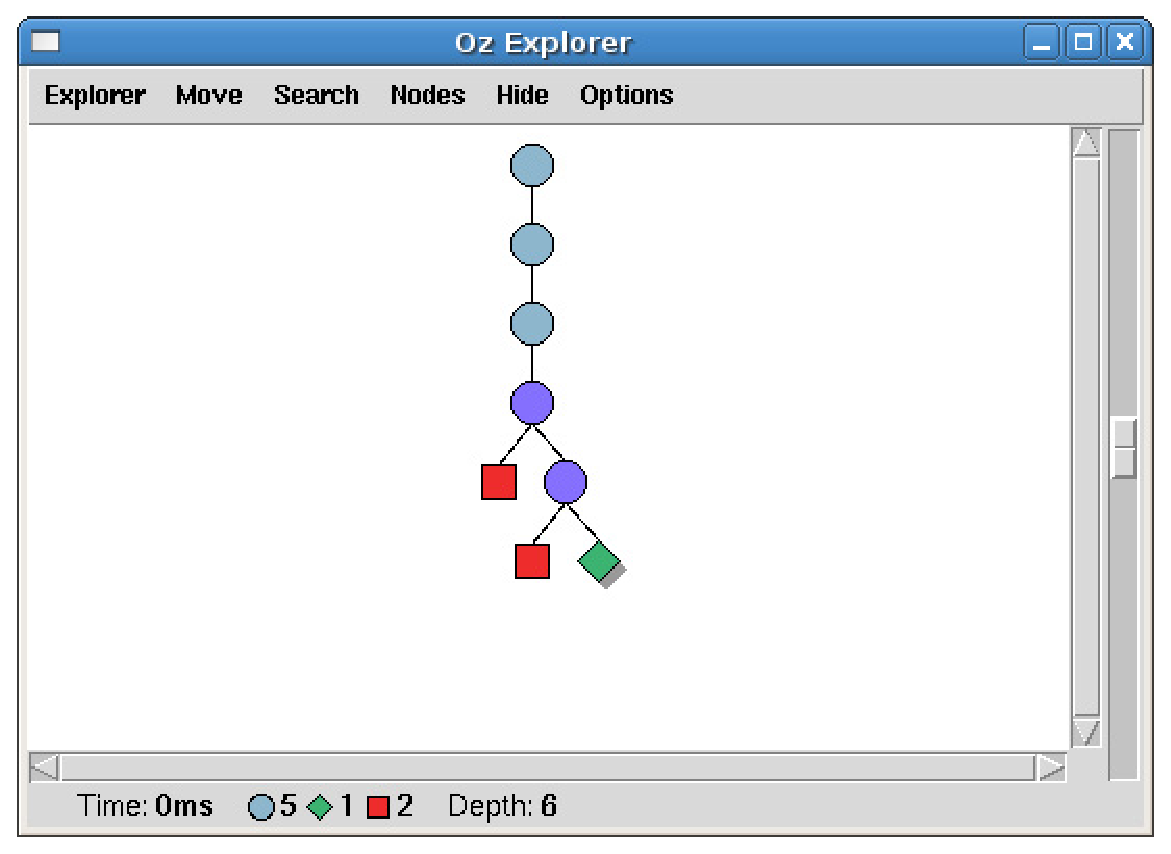
\includegraphics[scale=0.3]{images/screenshoty/explorer.eps}
\end{center}
\end{figure}

\subsection{Benchmarks implementation}


\subsection{Subjective description}